% !TeX program = xelatex
\documentclass[a4paper,10pt]{article}

% ============================================================================
% សន្លឹកកិច្ចការសិស្សបំពេញចន្លោះ ស-ខ្មៅ និងប្លង់ក្ដារខៀន/ចម្លើយគ្រូ (គ្មាន LCD / គ្មានកន្ត្រៃ)
% មេរៀនទី៥ (៣.២)៖ ពន្លាតគូបនៃទ្វេធា a^3+-b^3 និងត្រីកោណប៉ាស្កាល់ — ត្រូវគ្នានឹង LS_Plan_ALG56.tex
% ============================================================================
\usepackage[a4paper, left=1.0cm, right=1.0cm, top=0.75cm, bottom=1.00cm, footskip=0.52cm]{geometry}
\usepackage{amsmath}
\usepackage{unicode-math}
\usepackage{fontspec}
\usepackage{array, colortbl}
\usepackage[table]{xcolor}
\usepackage{enumitem}
\usepackage{pifont}
\usepackage{fancyhdr}
\usepackage{lastpage}
\usepackage{tikz}
\usepackage[most]{tcolorbox}
\usetikzlibrary{calc, arrows.meta, decorations.pathreplacing, positioning, babel}

\makeatletter
\let\@expl@@@mark@update@singlecol@structures@@\relax
\makeatother

\providecommand{\NGSFindFonts}{%
  \IfFileExists{C:/Windows/Fonts/cambria.ttc}{%
    \def\NGSSysPath{C:/Windows/Fonts/}%
    \def\NGSUserPath{C:/Users/KIT/AppData/Local/Microsoft/Windows/Fonts/}%
  }{%
    \IfFileExists{./fonts/KhmerOSsiemreap.ttf}{\def\NGSSysPath{./fonts/}\def\NGSUserPath{./fonts/}}{%
    \IfFileExists{../fonts/KhmerOSsiemreap.ttf}{\def\NGSSysPath{../fonts/}\def\NGSUserPath{../fonts/}}{%
    \IfFileExists{../../fonts/KhmerOSsiemreap.ttf}{\def\NGSSysPath{../../fonts/}\def\NGSUserPath{../../fonts/}}{%
    \IfFileExists{../../../fonts/KhmerOSsiemreap.ttf}{\def\NGSSysPath{../../../fonts/}\def\NGSUserPath{../../../fonts/}}{%
    \IfFileExists{../../../../fonts/KhmerOSsiemreap.ttf}{\def\NGSSysPath{../../../../fonts/}\def\NGSUserPath{../../../../fonts/}}{%
    \IfFileExists{../../../../../fonts/KhmerOSsiemreap.ttf}{\def\NGSSysPath{../../../../../fonts/}\def\NGSUserPath{../../../../../fonts/}}{%
    \IfFileExists{../../../../../../fonts/KhmerOSsiemreap.ttf}{\def\NGSSysPath{../../../../../../fonts/}\def\NGSUserPath{../../../../../../fonts/}}{%
      \def\NGSSysPath{../../../../../../../fonts/}\def\NGSUserPath{../../../../../../../fonts/}%
    }}}}}}}%
  }%
}
\NGSFindFonts

\setmathfont[Path={\NGSSysPath}, FontIndex=1, Scale=1.02]{cambria.ttc}
\defaultfontfeatures{Ligatures=TeX}

\setmainfont[
  Path={\NGSUserPath}, Extension=.ttf, Script=Khmer,
  BoldFont={KhmerOSsiemreap}, BoldFeatures={FakeBold=1.8},
  ItalicFont={KhmerOSsiemreap}, ItalicFeatures={FakeSlant=0.25},
  BoldItalicFont={KhmerOSsiemreap}, BoldItalicFeatures={FakeBold=1.8, FakeSlant=0.25}
]{KhmerOSsiemreap}

\newfontfamily\muol[Path={\NGSUserPath}, Extension=.ttf, Script=Khmer]{KhmerOSmuollight}
\newfontfamily\TimesEn[Path={\NGSSysPath}, Extension=.ttf, BoldFont={timesbd}, ItalicFont={timesi}, BoldItalicFont={timesbi}]{times}
\newfontfamily\CalibriFont[Path={\NGSSysPath}, Extension=.ttf]{calibri}

\XeTeXlinebreaklocale "km"
\XeTeXlinebreakskip = 0pt plus 1pt minus 0.1pt

\definecolor{panelgray}{gray}{0.94}
\definecolor{headgray}{gray}{0.85}

\pagestyle{fancy}
\fancyhf{}
\renewcommand{\headrulewidth}{0pt}
\fancyfoot[L]{\fontsize{7.4pt}{9.5pt}\selectfont អនុវិទ្យាល័យព្រះក្រសាំង \en{|} គ្រូ៖ ហុក ប៊ុនថែន \en{|} មេរៀនទី៥ (៣.២) គូបនៃទ្វេធានិងត្រីកោណប៉ាស្កាល់ \en{|} ថ្ងៃព្រហស្បតិ៍ ទី១០ ខែធ្នូ ឆ្នាំ២០២៦}
\fancyfoot[R]{\fontsize{7.8pt}{10pt}\selectfont ទំព័រ \en{\thepage\ / \pageref{LastPage}}}

\setlength{\parindent}{0pt}
\setlength{\parskip}{0pt}
\setlength{\tabcolsep}{4pt}

\newcommand{\en}[1]{{\TimesEn #1}}
\newcommand{\enbf}[1]{{\TimesEn\bfseries #1}}
\newcommand{\unit}[1]{\,\text{\en{#1}}}
\newcommand{\riel}{\,\text{៛}}
\newcommand{\cnum}[1]{\mbox{\fontsize{10pt}{12pt}\selectfont\ding{\numexpr181+#1\relax}}}
\newcommand{\chkbox}{\tikz[baseline=-0.15ex]\draw[black, line width=0.85pt, fill=white] (0,0) rectangle (0.24cm,0.24cm);}
\newcommand{\ansbox}[1][2.0cm]{\,\tikz[baseline=-0.65ex]\draw[black, line width=0.65pt, fill=white] (0,0) rectangle (#1, 0.42cm);\,}
\newcommand{\dotline}[1][2.2cm]{\makebox[#1]{\dotfill}}

\newcommand{\pagebanner}[2]{%
  \begin{tcolorbox}[
    enhanced, sharp corners, colback=headgray, colframe=black,
    boxrule=1.05pt, boxsep=1pt, top=2.5pt, bottom=2.5pt, left=6pt, right=6pt,
    after skip=3.5pt
  ]
    {\muol\fontsize{9.0pt}{13.2pt}\selectfont #1}\hfill{\fontsize{8.0pt}{11.2pt}\selectfont\textbf{#2}}
  \end{tcolorbox}%
}

\newcommand{\secstrip}[2]{%
  \vspace{3pt}%
  \begin{tcolorbox}[
    enhanced, sharp corners, colback=panelgray, colframe=black,
    boxrule=0.8pt, boxsep=0.8pt, top=2pt, bottom=2pt, left=5pt, right=5pt,
    after skip=3pt
  ]
    {\muol\fontsize{8.5pt}{12.2pt}\selectfont #1}\hfill{\fontsize{7.8pt}{10.8pt}\selectfont\textit{#2}}
  \end{tcolorbox}%
}

\newcolumntype{L}[1]{>{\raggedright\arraybackslash}p{#1}}
\newcolumntype{C}[1]{>{\centering\arraybackslash}p{#1}}

\begin{document}
\fontsize{9.5pt}{14.5pt}\selectfont

% ============================================================================
% ទំព័រទី ១៖ សន្លឹកកិច្ចការសិស្ស (ផ្នែកមុខ៖ E1 -> E2 -> E3)
% ============================================================================
\pagebanner{សន្លឹកកិច្ចការសិស្ស \enbf{(}៥\enbf{.}៣\enbf{.}២ គូបនៃទ្វេធា និងត្រីកោណប៉ាស្កាល់\enbf{)} \enbf{--} ផ្នែកមុខ}{ថ្នាក់ទី៨ \en{|} ទំ.៦៦--៦៨}

\begin{tcolorbox}[
  enhanced, sharp corners, colback=white, colframe=black,
  boxrule=0.8pt, boxsep=1.5pt, top=3.5pt, bottom=3.5pt, left=5pt, right=5pt,
  after skip=4pt
]
  \fontsize{9.0pt}{13.0pt}\selectfont
  \textbf{ឈ្មោះសិស្ស៖} \dotline[4.3cm] \quad
  \textbf{សមាជិកក្រុម៖} \dotline[4.3cm] \quad
  \textbf{ថ្នាក់ទី៖} ៨\dotline[0.9cm] \quad
  \textbf{ក្រុមទី៖} \dotline[1.0cm]
\end{tcolorbox}

% --- E1 Engage ---
\secstrip{ផ្នែកទី ១ \enbf{(E1 - Engage)} ៖ បេសកកម្មអន្ទាក់គូបនៃទ្វេធា $(x + 1)^3$}{រយៈពេល ៣ នាទី (គូស \ding{51} ក្នុង \chkbox)}

\begin{tcolorbox}[
  enhanced, sharp corners, colback=white, colframe=black,
  boxrule=0.8pt, boxsep=2.5pt, top=4pt, bottom=4pt, left=6pt, right=6pt
]
  គេចង់ពន្លាត $(x + 1)^3$ (ទំ.៦៦) ។ សាកជំនួស $x = 1$ បាន $(1 + 1)^3 = 2^3 = \mathbf{8}$ ។ តើសិស្សរូបណាពន្លាតបានត្រឹមត្រូវ?\\[3pt]
  \chkbox\ \textbf{សិស្ស ក៖} $(x + 1)^3 = x^3 + 1^3 = x^3 + 1$ \qquad
  \chkbox\ \textbf{សិស្ស ខ៖} $(x + 1)^3 = (x + 1)^2(x + 1) = x^3 + 3x^2 + 3x + 1$\\[3pt]
  $\bullet$ \textbf{តេស្តដោយ $x = 1$៖} កន្សោមសិស្ស ក ស្មើ $1 + 1 =$ \dotline[1.2cm]; \ ឯកន្សោមសិស្ស ខ ស្មើ $1 + 3 + 3 + 1 =$ \dotline[1.2cm] ។
\end{tcolorbox}

\vspace{3pt}

% --- E2 Explore ---
\secstrip{ផ្នែកទី ២ \enbf{(E2 - Explore)} ៖ គូបនៃទ្វេធា ផលដក/បូកគូប និងត្រីកោណប៉ាស្កាល់ (ទំ.៦៦--៦៨)}{រយៈពេល ១១ នាទី}

\textbf{សកម្មភាព ១ (\en{E2-A} — ៦ នាទី)៖ កសាងរូបមន្ត $(a + b)^3$ និង $(a - b)^3$ (ទំ.៦៦--៦៧)}

\begin{tcolorbox}[
  enhanced, sharp corners, colback=white, colframe=black,
  boxrule=0.8pt, boxsep=2.5pt, top=4pt, bottom=4pt, left=6pt, right=6pt
]
  $\bullet$ \textbf{១) គូបនៃផលបូក៖} $(a+b)^3 = (a^2+2ab+b^2)(a+b) = a^3 + 2a^2b + ab^2 + a^2b + 2ab^2 + b^3 =$ \ansbox[4.6cm]\\[3pt]
  $\bullet$ \textbf{២) គូបនៃផលដក៖} $(a-b)^3 = (a-b)(a^2-2ab+b^2) = a^3 - 2a^2b + ab^2 - a^2b + 2ab^2 - b^3 =$ \ansbox[4.6cm]\\[3pt]
  $\bullet$ \textbf{៣) អនុវត្តភ្លាម (លំហាត់គំរូ ទំ.៦៧)៖} $(x - 1)^3 =$ \dotline[4.8cm] ។
\end{tcolorbox}

\vspace{4pt}
\textbf{សកម្មភាព ២ (\en{E2-B} — ៥ នាទី)៖ ពន្លាត $(a\mp b)(a^2\pm ab+b^2)$ និងត្រីកោណប៉ាស្កាល់ (ទំ.៦៧--៦៨)}

\begin{tcolorbox}[
  enhanced, sharp corners, colback=white, colframe=black,
  boxrule=0.8pt, boxsep=2.5pt, top=4pt, bottom=4pt, left=6pt, right=6pt
]
  \begin{minipage}[c]{5.2cm}
    \centering
    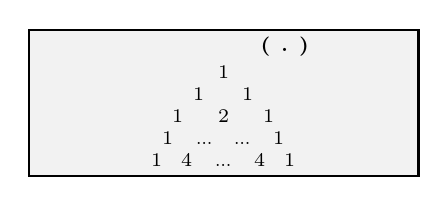
\begin{tikzpicture}[x=1cm, y=1cm, every node/.style={font=\scriptsize, text=black}]
      \draw[black, line width=0.75pt, fill=gray!10] (0,0) rectangle (4.95,1.85);
      \node at (2.475,1.64) {\textbf{បំពេញត្រីកោណប៉ាស្កាល់ (ទំ.៦៨)}};
      \node at (2.475,1.32) {$1$};
      \node at (2.475,1.04) {$1 \qquad 1$};
      \node at (2.475,0.76) {$1 \quad\ \ 2 \quad\ \ 1$};
      \node at (2.475,0.48) {$1 \quad \ldots \quad \ldots \quad 1$};
      \node at (2.475,0.20) {$1 \quad 4 \quad \ldots \quad 4 \quad 1$};
    \end{tikzpicture}
  \end{minipage}\hfill
  \begin{minipage}[c]{12.8cm}
    $\bullet$ \textbf{១) ផលដកគូប (ទំ.៦៧)៖} $(a - b)(a^2 + ab + b^2) =$ \ansbox[3.0cm]\\[3pt]
    \hspace*{0.3cm}លំហាត់គំរូ៖ $(x - 1)(x^2 + x + 1) =$ \dotline[2.6cm]\\[3pt]
    $\bullet$ \textbf{២) ផលបូកគូប (ទំ.៦៧)៖} $(a + b)(a^2 - ab + b^2) =$ \ansbox[3.0cm]\\[3pt]
    \hspace*{0.3cm}លំហាត់គំរូ៖ $(x + 1)(x^2 - x + 1) =$ \dotline[2.6cm]
  \end{minipage}
\end{tcolorbox}

\vfill

% --- E3 Explain ---
\secstrip{ផ្នែកទី ៣ \enbf{(E3 - Explain)} ៖ រូបមន្តសង្ខេបទាំង ៤ និងធនាគារហេតុផល \enbf{B\&W}}{រយៈពេល ៦ នាទី}

\begin{tcolorbox}[
  enhanced, sharp corners, colback=white, colframe=black,
  boxrule=0.85pt, boxsep=2.5pt, top=4pt, bottom=4pt, left=6pt, right=6pt
]
  $\bullet$ \textbf{(4)} $(a + b)^3 =$ \ansbox[4.6cm] \qquad
  \textbf{(5)} $(a - b)^3 =$ \ansbox[4.6cm]\\[4pt]
  $\bullet$ \textbf{(6)} $(a - b)(a^2 + ab + b^2) =$ \ansbox[3.0cm] \qquad
  \textbf{(7)} $(a + b)(a^2 - ab + b^2) =$ \ansbox[3.0cm]\\[4pt]
  \tikz\draw[black, dashed, line width=0.5pt] (0,0) -- (18.4cm,0);\\[3pt]
  \fontsize{8.8pt}{13.0pt}\selectfont
  \textbf{ធនាគារហេតុផល (\en{Warrant Bank})៖} \quad
  \cnum{1} មេគុណគូបទ្វេធាគឺ $1, 3, 3, 1$ \quad
  \cnum{2} សញ្ញា $(a-b)^3$ ឆ្លាស់គ្នា $+, -, +, -$\\
  \cnum{3} ត្រីធាក្នុង $a^3\mp b^3$ គឺ $a^2 \pm ab + b^2$ (គ្មាន $2ab$) \quad
  \cnum{4} ត្រីកោណប៉ាស្កាល់៖ តួកណ្ដាលស្មើផលបូកពីរតួខាងលើជាប់គ្នា
\end{tcolorbox}

% ============================================================================
% ទំព័រទី ២៖ សន្លឹកកិច្ចការសិស្ស (ផ្នែកខាងខ្នង៖ E4 -> E5 -> កិច្ចការផ្ទះ)
% ============================================================================
\clearpage
\pagebanner{សន្លឹកកិច្ចការសិស្ស \enbf{(}៥\enbf{.}៣\enbf{.}២ គូបនៃទ្វេធា និងត្រីកោណប៉ាស្កាល់\enbf{)} \enbf{--} ផ្នែកខាងខ្នង}{ថ្នាក់ទី៨ \en{|} ទំ.៦៦--៦៨, ៧៣}

% --- E4 Elaborate ---
\secstrip{ផ្នែកទី ៤ \enbf{(E4 - Elaborate)} ៖ លំហាត់គំរូពង្រីកគូបទ្វេធា ផលគុណ $a^3\pm b^3$ និង $(x+1)^4$}{រយៈពេល ១០ នាទី}

\begin{tcolorbox}[
  enhanced, sharp corners, colback=white, colframe=black,
  boxrule=0.8pt, boxsep=2.5pt, top=4pt, bottom=4pt, left=6pt, right=6pt
]
  \textbf{១) ពន្លាតគូបនៃទ្វេធាមានមេគុណ (ប្រតិបត្តិទំ.៦៦--៦៧)៖}\\[3pt]
  \hspace*{0.3cm}$\bullet$ $(x + 2y)^3 = x^3 + 3x^2(2y) + 3x(2y)^2 + (2y)^3 =$ \ansbox[5.8cm]\\[3pt]
  \hspace*{0.3cm}$\bullet$ $(3x - 2y)^3 = (3x)^3 - 3(3x)^2(2y) + 3(3x)(2y)^2 - (2y)^3 =$ \ansbox[5.8cm]\\[5pt]
  \textbf{២) ពន្លាតផលគុណ $a^3\pm b^3$ និងប្រើត្រីកោណប៉ាស្កាល់ (ទំ.៦៧--៦៨)៖}\\[3pt]
  \hspace*{0.3cm}$\bullet$ $(2x - 1)(4x^2 + 2x + 1) =$ \ansbox[3.2cm] \qquad
  $\bullet$ $(x + 3)(x^2 - 3x + 9) =$ \ansbox[3.2cm]\\[3pt]
  \hspace*{0.3cm}$\bullet$ ប្រើជួរទី៤ ($1, 4, 6, 4, 1$) នៃត្រីកោណប៉ាស្កាល់៖ $(x + 1)^4 =$ \ansbox[6.2cm]\\[3pt]
  \fontsize{8.8pt}{13.0pt}\selectfont
  \textbf{ឆ្លុះបញ្ចាំង (\en{EIA Looking-Back})៖} តើ $(a-b)(a^2+2ab+b^2)$ ស្មើ $a^3-b^3$ ដែរឬទេ? \textbf{ចម្លើយ៖} \dotline[5.2cm] ។
\end{tcolorbox}

\vspace{4pt}

% --- E5 Evaluate ---
\secstrip{ផ្នែកទី ៥ \enbf{(E5 - Evaluate)} ៖ ប្រតិបត្តិ (ទំ.៦៦--៦៧) សំណួរវិនិច្ឆ័យ \enbf{A--D} និងសំបុត្រចេញ}{រយៈពេល ១០ នាទី}

\begin{tcolorbox}[
  enhanced, sharp corners, colback=white, colframe=black,
  boxrule=0.8pt, boxsep=2.5pt, top=4pt, bottom=4pt, left=6pt, right=6pt
]
  \textbf{១) ប្រតិបត្តិជាក្រុម (ទំ.៦៦--៦៧)៖}\\[3pt]
  \hspace*{0.3cm}$\bullet$ ទំ.៦៦ (ខ)៖ $(x + 3y)^3 =$ \ansbox[5.8cm]\\[3pt]
  \hspace*{0.3cm}$\bullet$ ទំ.៦៧ (ខ)៖ $(2x - y)^3 =$ \ansbox[5.2cm] \quad
  ទំ.៦៧ ក្រោម (គ)៖ $(2x+1)(4x^2-2x+1) =$ \ansbox[2.4cm]\\[4pt]
  \textbf{២) បិទបេសកកម្ម \en{E1}៖} សិស្ស \dotline[1.0cm] ត្រឹមត្រូវ ព្រោះ $(x + 1)^3 =$ \ansbox[4.8cm] ។
\end{tcolorbox}

\vspace{4pt}

\begin{tcolorbox}[
  enhanced, sharp corners, colback=white, colframe=black,
  boxrule=0.8pt, boxsep=2.5pt, top=4pt, bottom=4pt, left=6pt, right=6pt
]
  \textbf{៣) សំណួរវិនិច្ឆ័យ \en{A--D} (ពន្លាតគូបនៃទ្វេធា $(x - 2)^3$ — គូសរង្វង់ រួចលើកម្រាមដៃ ១--៤)៖}\\[3pt]
  \textbf{\en{A.}} $x^3 - 8$ \quad
  \textbf{\en{B.}} $x^3 - 6x^2 + 12x - 8$ \quad
  \textbf{\en{C.}} $x^3 - 6x^2 - 12x - 8$ \quad
  \textbf{\en{D.}} $x^3 - 2x^2 + 4x - 8$\\[4pt]
  \tikz\draw[black, dashed, line width=0.5pt] (0,0) -- (18.4cm,0);\\[3pt]
  \textbf{៤) សំបុត្រចេញ ៦០ វិនាទី (ទំ.៦៧ ខ)៖} ពន្លាត $(x - 3)(x^2 + 3x + 9) =$ \ansbox[3.6cm] ។
\end{tcolorbox}

\vfill

% --- Homework ---
\begin{tcolorbox}[
  enhanced, sharp corners, colback=panelgray, colframe=black,
  boxrule=0.95pt, boxsep=2pt, top=3.5pt, bottom=3.5pt, left=6pt, right=6pt
]
  {\muol\fontsize{9.0pt}{13.0pt}\selectfont កិច្ចការផ្ទះ \enbf{(}សៀវភៅគោល ទំ.៦៦--៦៧ និង ទំ.៧៣ លេខ ១០ គ, ឃ, ង\enbf{)}}\\[2.5pt]
  \fontsize{8.8pt}{13.0pt}\selectfont
  $\bullet$ \textbf{១) ប្រតិបត្តិទំ.៦៦ (គ, ឃ) និង ទំ.៦៧ (ឃ)៖} ពន្លាត $(3x+4y)^3$, $\left(\dfrac{1}{5}a+b\right)^3$, $\left(\dfrac{1}{5}t-k\right)^3$ និង $(\sqrt{2}a-3b)(2a^2+3\sqrt{2}ab+9b^2)$ ។\\
  $\bullet$ \textbf{២) ទំ.៧៣ \#10 គ, ឃ, ង៖} ពន្លាតនិងបង្រួម $(a-3b)^2+9(a^2-3b)+5$, $-x(4x-3y)+x^2-12xy$ និង $(x-1)^3 - (x+2)^3$ ។
\end{tcolorbox}

% ============================================================================
% ទំព័រទី ៣៖ ទំព័រគ្រូបង្រៀន (គំរូប្លង់ក្ដារខៀន ៣ ផ្នែក + ចម្លើយផ្ទៀងផ្ទាត់រហ័ស)
% ============================================================================
\clearpage
\pagebanner{ទំព័រគ្រូបង្រៀន ៖ ប្លង់ក្ដារខៀន \enbf{(}គ្មាន \enbf{LCD)} និងចម្លើយផ្ទៀងផ្ទាត់រហ័ស}{៥.៣.២ គូបនៃទ្វេធា និងត្រីកោណប៉ាស្កាល់ (\en{ALG56})}

\secstrip{១. គំរូប្លង់បែងចែកក្ដារខៀន ៣ ផ្នែក សម្រាប់ថ្នាក់រៀនគ្មាន \enbf{LCD}}{សម្រាប់គ្រូប្រើដីស/ហ្វឺត}

\begin{center}
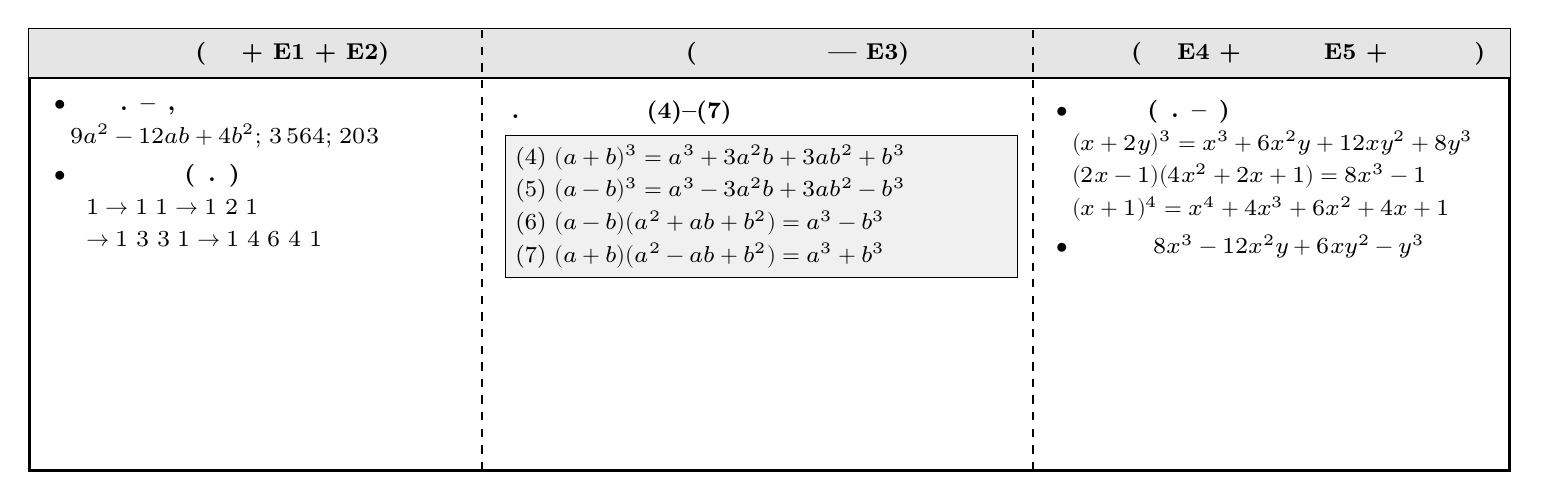
\begin{tikzpicture}[x=1cm, y=1cm, every node/.style={font=\fontsize{8.3pt}{11.8pt}\selectfont, text=black}]
  \draw[black, line width=1.1pt] (0,0) rectangle (18.8,5.60);
  \fill[gray!20] (0,4.98) rectangle (18.8,5.60);
  \draw[black, line width=0.7pt] (0,4.98) -- (18.8,4.98);
  \draw[black, dashed, line width=0.7pt] (5.75,0) -- (5.75,5.60);
  \draw[black, dashed, line width=0.7pt] (12.75,0) -- (12.75,5.60);

  \node at (2.875,5.29) {\textbf{ផ្នែកឆ្វេង (កំណែ + \en{E1} + \en{E2})}};
  \node at (9.25,5.29) {\textbf{ផ្នែកកណ្ដាល (ខ្លឹមសារគោលរក្សាទុក — \en{E3})}};
  \node at (15.775,5.29) {\textbf{ផ្នែកស្ដាំ (គំរូ \en{E4} + ប្រតិបត្តិ \en{E5} + កិច្ចការផ្ទះ)}};

  % Left
  \node[anchor=north west, text width=5.35cm] at (0.20,4.82) {%
    $\bullet$ \textbf{កំណែ ទំ.៦៤--៦៥, ៧៣៖}\\
    \hspace*{0.2cm}$9a^2-12ab+4b^2$; $3\,564$; $203$\\[2pt]
    $\bullet$ \textbf{ត្រីកោណប៉ាស្កាល់ (ទំ.៦៨)៖}\\
    \hspace*{0.4cm}$1 \to 1\ 1 \to 1\ 2\ 1$\\
    \hspace*{0.4cm}$\to 1\ 3\ 3\ 1 \to 1\ 4\ 6\ 4\ 1$
  };

  % Center
  \node[anchor=north west, text width=6.65cm] at (5.92,4.82) {%
    {\muol\fontsize{8.5pt}{12pt}\selectfont ៣\enbf{.}២ រូបមន្តគូបសង្ខេប \enbf{(4)--(7)}}\\[3pt]
    \tikz\node[draw=black, fill=gray!12, inner sep=3.5pt, text width=6.25cm]{%
      (4) $(a+b)^3 = a^3 + 3a^2b + 3ab^2 + b^3$\\
      (5) $(a-b)^3 = a^3 - 3a^2b + 3ab^2 - b^3$\\
      (6) $(a-b)(a^2+ab+b^2) = a^3 - b^3$\\
      (7) $(a+b)(a^2-ab+b^2) = a^3 + b^3$
    };
  };

  % Right
  \node[anchor=north west, text width=5.8cm] at (12.92,4.82) {%
    $\bullet$ \textbf{លំហាត់គំរូ (ទំ.៦៦--៦៨)៖}\\
    \hspace*{0.2cm}$(x+2y)^3 = x^3+6x^2y+12xy^2+8y^3$\\
    \hspace*{0.2cm}$(2x-1)(4x^2+2x+1) = 8x^3-1$\\
    \hspace*{0.2cm}$(x+1)^4 = x^4+4x^3+6x^2+4x+1$\\[2pt]
    $\bullet$ \textbf{ប្រតិបត្តិ៖} $8x^3-12x^2y+6xy^2-y^3$
  };
\end{tikzpicture}
\end{center}

\vspace{4pt}
\secstrip{២. ចម្លើយផ្ទៀងផ្ទាត់រហ័សសម្រាប់សន្លឹកកិច្ចការសិស្ស \enbf{(}ទំព័រ ១ និង ទំព័រ ២\enbf{)}}{\en{Answer Key}}

\begin{tcolorbox}[
  enhanced, sharp corners, colback=white, colframe=black,
  boxrule=0.8pt, boxsep=2pt, top=4pt, bottom=4pt, left=6pt, right=6pt
]
  \fontsize{9.0pt}{13.5pt}\selectfont
  $\bullet$ \textbf{ផ្នែក \en{E1}៖} \textbf{សិស្ស ខ} ត្រឹមត្រូវ ($x^3+3x^2+3x+1$) ព្រោះពេល $x=1$ បាន $1+3+3+1 = 8 = 2^3$ ។\\[2pt]
  $\bullet$ \textbf{ផ្នែក \en{E2}៖} \textbf{សកម្មភាព ១៖} $a^3+3a^2b+3ab^2+b^3$; $a^3-3a^2b+3ab^2-b^3$; $x^3-3x^2+3x-1$ ។ \textbf{សកម្មភាព ២៖} ត្រីកោណប៉ាស្កាល់ $3, 3$ និង $6$; $a^3-b^3, x^3-1$; $a^3+b^3, x^3+1$ ។\\[2pt]
  $\bullet$ \textbf{ផ្នែក \en{E4}៖} ១) $x^3+6x^2y+12xy^2+8y^3$; $27x^3-54x^2y+36xy^2-8y^3$; ២) $8x^3-1$; $x^3+27$; $x^4+4x^3+6x^2+4x+1$ ។\\[2pt]
  $\bullet$ \textbf{ផ្នែក \en{E5}៖} ១) $x^3+9x^2y+27xy^2+27y^3$; $8x^3-12x^2y+6xy^2-y^3$; $8x^3+1$; ២) សិស្ស ខ; ៣) \textbf{ជម្រើស \en{B}} ($x^3-6x^2+12x-8$); ៤) $x^3-27$ ។
\end{tcolorbox}

\vspace{4pt}
\secstrip{៣. ចម្លើយលម្អិតនៃកិច្ចការផ្ទះ \enbf{(}សម្រាប់ផ្ទៀងនៅដើមម៉ោងបន្ទាប់ ៥\enbf{.}៤\enbf{.}១\enbf{)}}{សៀវភៅគោល ទំ.៦៦--៦៧, ៧៣}

\begin{tcolorbox}[
  enhanced, sharp corners, colback=white, colframe=black,
  boxrule=0.8pt, boxsep=2pt, top=4pt, bottom=4pt, left=6pt, right=6pt
]
  \fontsize{8.8pt}{13.2pt}\selectfont
  $\bullet$ \textbf{១) ទំ.៦៦–៦៧៖} $(3x+4y)^3 = \mathbf{27x^3+108x^2y+144xy^2+64y^3}$; \ $(\frac{1}{5}a+b)^3 = \mathbf{\frac{1}{125}a^3+\frac{3}{25}a^2b+\frac{3}{5}ab^2+b^3}$; \ $(\frac{1}{5}t-k)^3 = \mathbf{\frac{1}{125}t^3-\frac{3}{25}t^2k+\frac{3}{5}tk^2-k^3}$; \ $(\sqrt{2}a-3b)(2a^2+3\sqrt{2}ab+9b^2) = (\sqrt{2}a)^3-(3b)^3 = \mathbf{2\sqrt{2}a^3 - 27b^3}$ ។\\[2pt]
  $\bullet$ \textbf{២) ទំ.៧៣ \#10 គ៖} $\mathbf{10a^2-6ab+9b^2-27b+5}$; \ \textbf{ឃ៖} $\mathbf{-3x^2-9xy}$; \ \textbf{ង៖} $(x^3-3x^2+3x-1)-(x^3+6x^2+12x+8) = \mathbf{-9x^2-9x-9}$ ។
\end{tcolorbox}

\end{document}
